\section{The Detailed Pipeline}
\label{chap:detailed_pipeline}

\subsection{Proposal Scoring}
\label{detailed:proposal}

\begin{figure}[h]
\centering
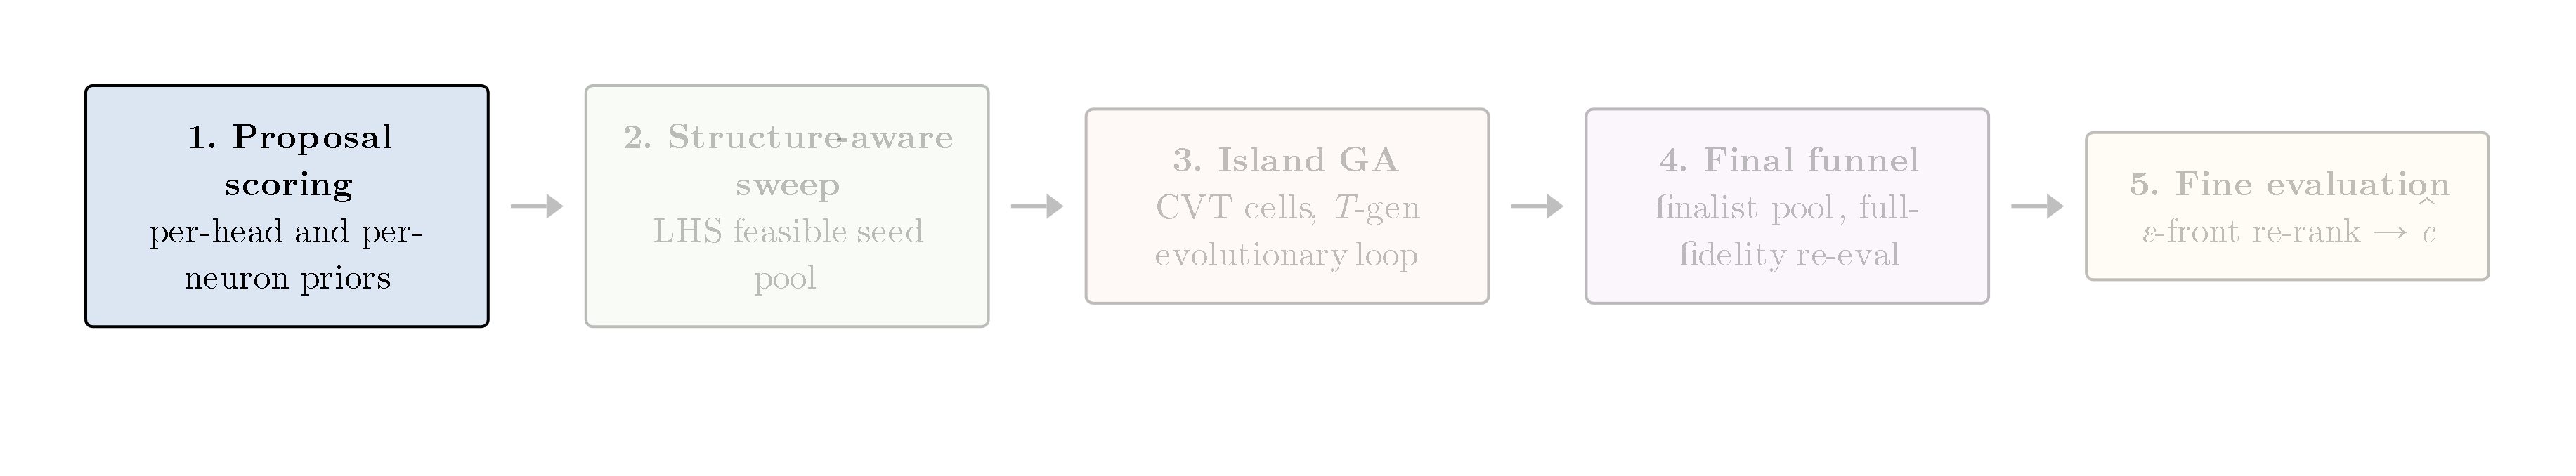
\includegraphics[width=0.85\linewidth]{figures/phase_banner_1.png}
\end{figure}

The first phase computes the priors that the operators of Phase~3 and the repair routine consume. The priors are per-head and per-neuron sensitivities of the teacher's per-layer residual update target, evaluated on the calibration set of Section~\ref{chap:calibration}.

For head $h$ of layer $\ell$, let $g_{\ell,h}(x)$ denote the gradient of the teacher-forced per-layer update target with respect to a multiplicative gate placed at head $(\ell, h)$, evaluated on a calibration example $x$. The head sensitivity score is
\[
s_H[\ell, h] \;=\; \mathbb{E}_{x \sim \mathcal{D}_{\mathrm{cal}}}\!\left[\, g_{\ell,h}(x)^2 \,\right] + \lambda \cdot \mathrm{MSE}\!\left( \widetilde\Delta^{(\teacher,\, h{=}0)}_{\ell}, \Dlt{\ell} \right),
\]
with $\lambda = 0.35$, where the MSE term measures the reconstruction error of the teacher's per-layer update when head $(\ell, h)$ is zeroed. The neuron score $s_N[\ell, n]$ is defined analogously over the gates of feed-forward neuron $(\ell, n)$. Both scores are row-normalised per layer so that across-depth differences in absolute gradient magnitude do not dominate the priors.

The per-layer aggregate
\[
\mathrm{imp}(\ell) \;=\; \sum_{h} s_H[\ell, h] \;+\; \sum_{n} s_N[\ell, n]
\]
gives a single importance number per layer, used in Phase~2 to choose which layers to activate and during repair to define the protected core.

Neuron addition and removal during repair act on blocks of size $b_n = 16$ rather than individual neurons. For each layer $\ell$, let $\pi_\ell$ be the permutation that sorts $s_N[\ell, \cdot]$ in descending order. The cumulative block-score table is
\[
S_\ell[b] \;=\; \sum_{j = 1}^{b \cdot b_n} s_N[\ell,\, \pi_\ell(j)], \qquad b = 0, 1, \ldots, \lfloor \nffn / b_n \rfloor.
\]
The marginal gain of adding the $(b{+}1)$-th block to layer $\ell$ is $S_\ell[b{+}1] - S_\ell[b]$, and the marginal loss of removing the $b$-th block is $S_\ell[b] - S_\ell[b{-}1]$, both available in $O(1)$ after the one-time descending sort.

\begin{figure}[h]
\centering
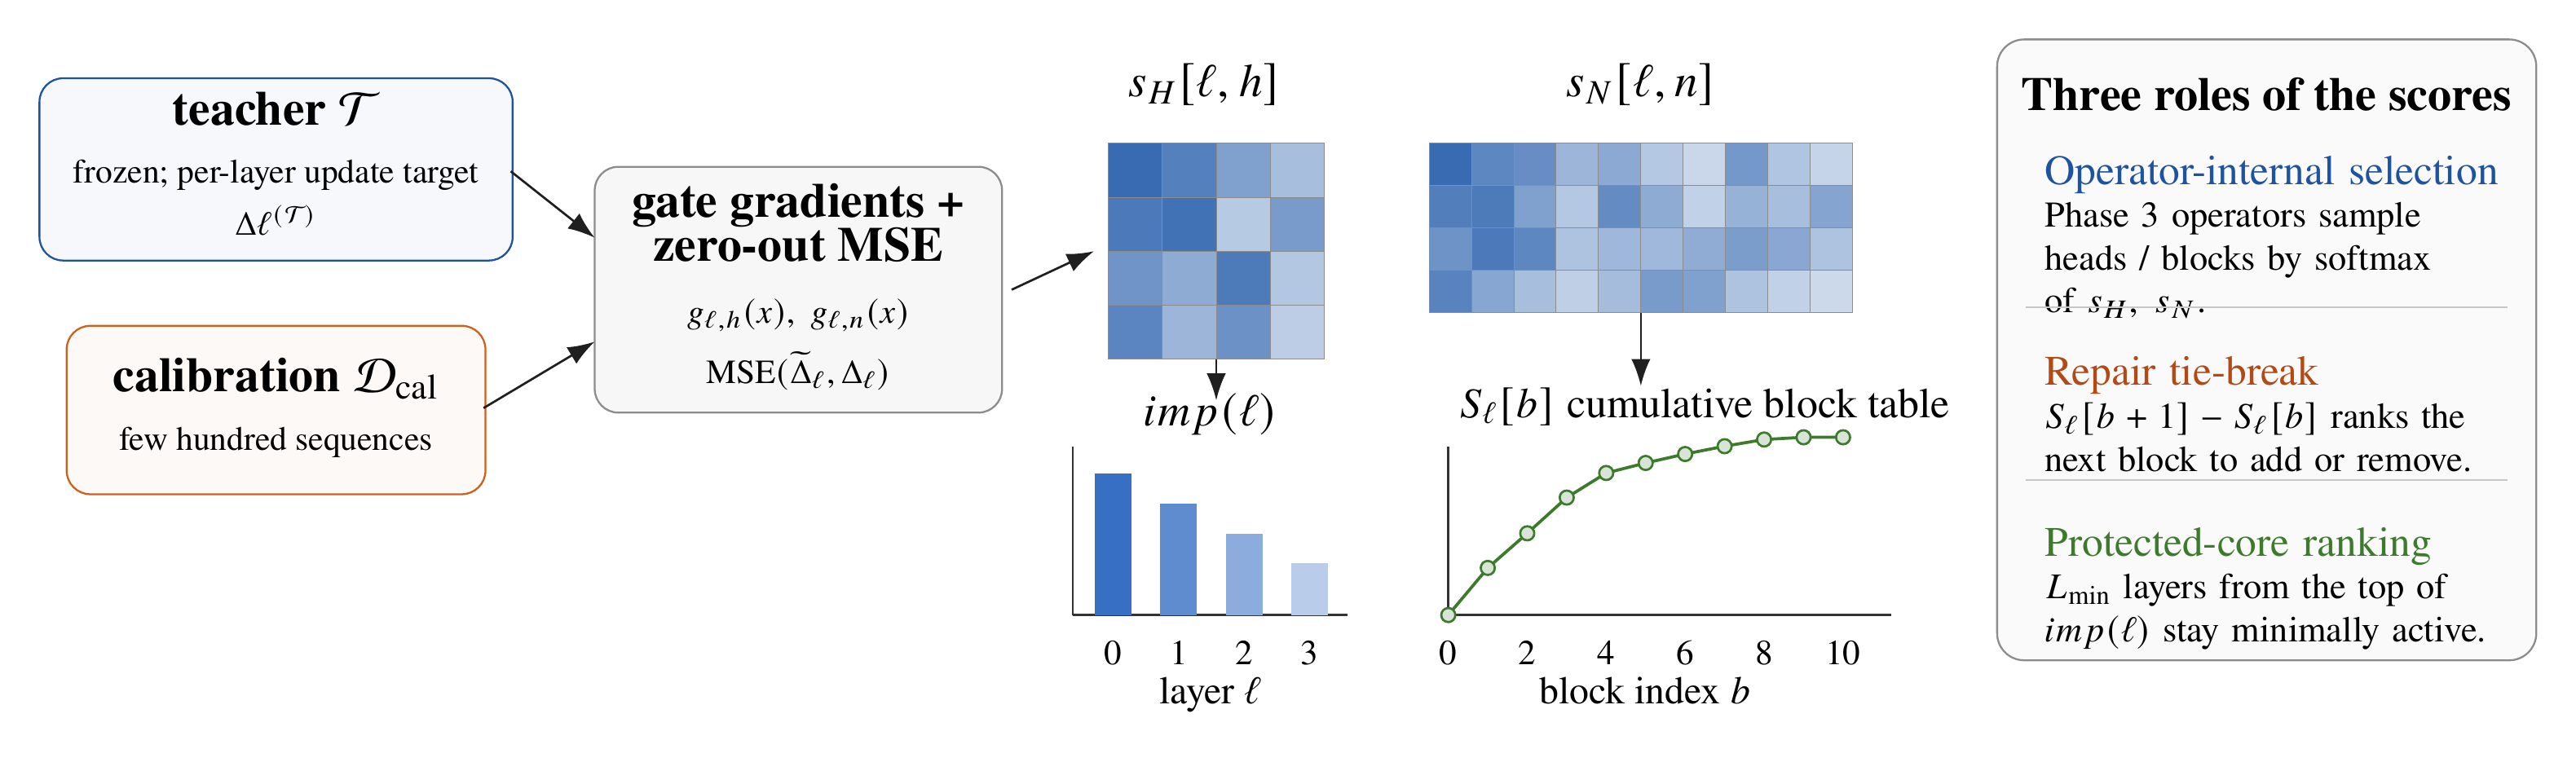
\includegraphics[width=0.95\linewidth]{figures/proposal_scoring.png}
\caption{Proposal scoring. For each calibration batch, gradients of the teacher's per-layer update target with respect to head and neuron gates yield squared sensitivities and a reconstruction MSE; their combination, row-normalised per layer, produces $s_H[\ell, h]$ and $s_N[\ell, n]$. Summing over each layer gives $\mathrm{imp}(\ell)$. Sorting $s_N[\ell, \cdot]$ in descending order and accumulating block sums yields the table $S_\ell[b]$, from which marginal gain and loss queries take $O(1)$.}
\label{fig:proposal_scoring}
\end{figure}

The scores serve three roles in the rest of the procedure. The operator-internal selection in Phase~3 samples heads and neuron blocks with probabilities derived from $s_H$ and $s_N$ when deciding which units to add or remove. The repair routine breaks ties between candidates of equal cost by preferring the addition of the highest-score block or the removal of the lowest-score block via $S_\ell$. The protected core during repair, namely the $L_{\min}$ layers that must remain at least minimally active, is drawn from the top of $\mathrm{imp}(\ell)$.


\subsection{Initialisation: Structure-Aware Sweep}
\label{detailed:sweep}

\begin{figure}[h]
\centering
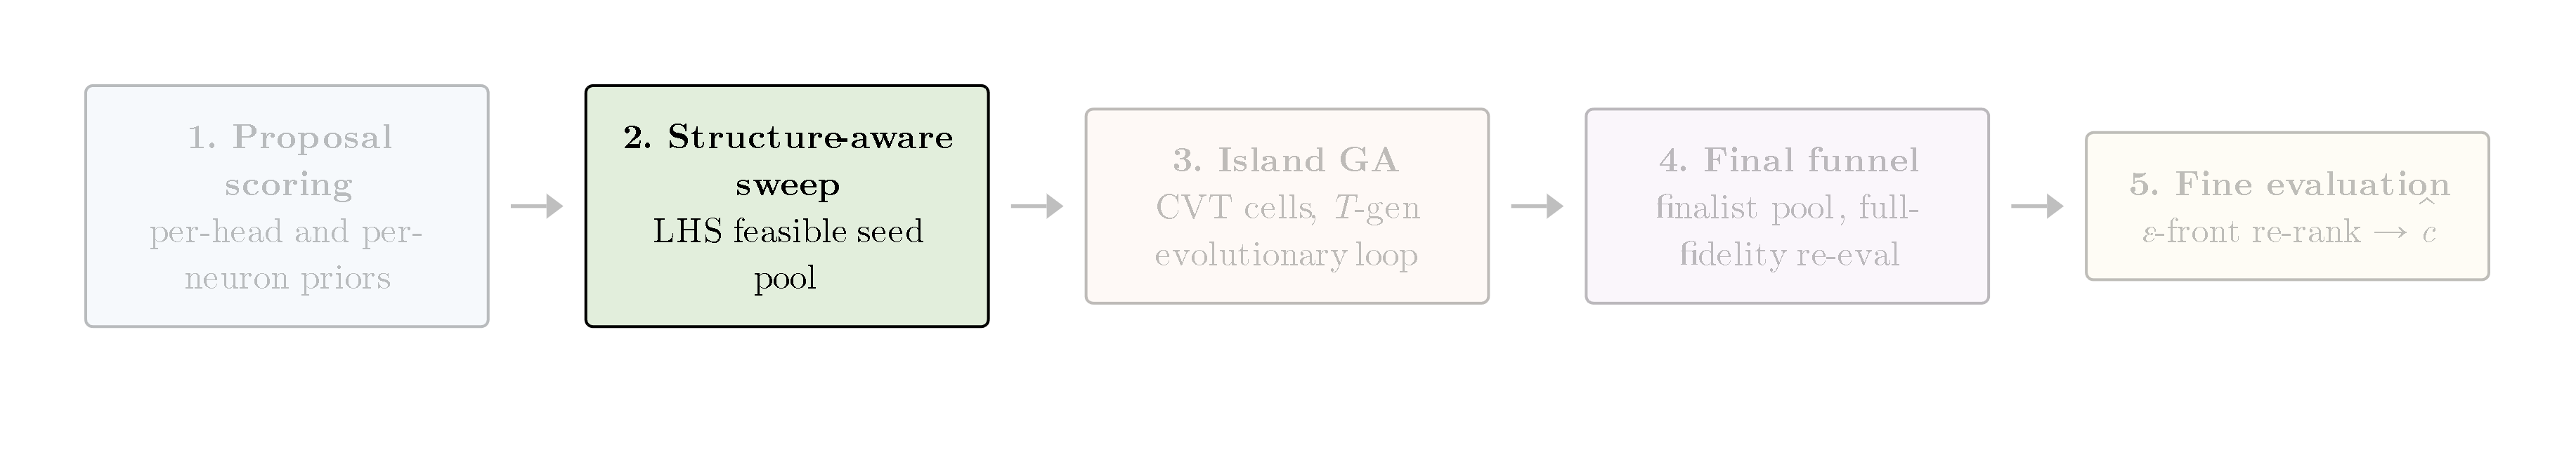
\includegraphics[width=0.85\linewidth]{figures/phase_banner_2.png}
\end{figure}

The second phase produces the pool of feasible candidates that will seed the per-region populations of Phase~3 and serve as the sample from which the partition of $\mathcal{X}_\budget$ into regions is fitted. The pool must cover the search space evenly along the macro descriptors that distinguish architecturally different masks; uniform sampling does this poorly because it concentrates draws away from the corners of the descriptor space. The sweep replaces uniform sampling by a stratified Latin hypercube design over three macro axes, in which every level of each axis appears the same number of times, and produces one candidate per grid cell by a deterministic construction that draws on the priors of the preceding subsection.

The first axis is the active-layer count $\nactive$, ranging over $\{L_{\min}, \ldots, L_{\max}\}$, where $L_{\min}$ is the active-depth floor of the search and $L_{\max} = \lfloor \budget / (\headcost + b_n \neuroncost) \rfloor$ is the largest depth at which the minimum-cost feasible candidate still fits the budget. The second axis is the head-MAC fraction $\phi_H \in \{0.05, 0.10, 0.15, 0.25, 0.35, 0.50, 0.65, 0.80, 0.92\}$, which controls how the budget is split between attention and feed-forward capacity and ranges from neuron-dominated to attention-dominated configurations. The third axis is a subset mode that selects which $\nactive$ layers are kept active given the importance vector $\mathrm{imp}(\ell)$, drawn from $\{\mathtt{topk}, \mathtt{noisy\_topk}, \mathtt{weighted}, \mathtt{random}\}$. The subset mode may optionally be paired with a partial-layer style that injects single-branch layers (attention-only or feed-forward-only) into the sweep pool, which broadens coverage without enlarging the grid.

The four subset modes differ in how much they trust the importance prior. The $\mathtt{topk}$ mode restricts attention to the $\lceil 1.75 \nactive \rceil$ layers with the largest $\mathrm{imp}(\ell)$ and then samples $\nactive$ of them with multinomial weights proportional to $\mathrm{imp}(\ell)$. The $\mathtt{noisy\_topk}$ mode perturbs $\mathrm{imp}$ by independent Gaussian noise of standard deviation $0.30$ and takes the top $\nactive$ of the perturbed vector, which lets layers ranked just below the top occasionally win and so injects mild diversity. The $\mathtt{weighted}$ mode samples $\nactive$ layers without replacement from a multinomial proportional to $\mathrm{imp}(\ell) \cdot \exp(0.20 \cdot \mathcal{N}(0, 1))$, treating $\mathrm{imp}(\ell)$ as a soft preference rather than a strict ordering. The $\mathtt{random}$ mode ignores the prior entirely and returns a uniform random subset of size $\nactive$, providing a control against the priors of Section~\ref{detailed:proposal} dominating the seed pool.

Given a grid cell $(\nactive, \phi_H, \mathrm{mode})$, the construction first calls the subset mode to obtain the active set $A \subset \{1, \ldots, \nlayers\}$, then divides the budget across the layers of $A$ by importance-proportional weights perturbed by lognormal noise,
\[
w_\ell \;=\; \mathrm{imp}(\ell) \cdot \exp(0.35 \cdot \xi_\ell), \quad \xi_\ell \sim \mathcal{N}(0, 1), \qquad \tilde w_\ell \;=\; w_\ell \,\big/\, \textstyle \sum_{k \in A} w_k,
\]
so that layers of similar importance still receive slightly different shares across cells. The cell's choice of $\phi_H$ then sets the head and neuron spends to $\phi_H \budget$ and $(1 - \phi_H) \budget$ respectively, and the active head count and neuron count at layer $\ell \in A$ follow from these shares,
\[
\actl \;=\; \mathrm{round}\!\big( \phi_H \budget \, \tilde w_\ell / \headcost \big), \qquad
\nactl \;=\; b_n \cdot \big\lfloor (1 - \phi_H) \budget \, \tilde w_\ell / (b_n \neuroncost) \big\rfloor,
\]
with $\actl$ clipped to $[1, \nheads]$ and $\nactl$ to $[b_n, \nffn]$. The specific heads retained at layer $\ell$ are then sampled from a temperature-softmax of $s_H[\ell, \cdot]$ at temperature $\tau \sim \mathrm{Unif}[0.55, 1.10]$, so layers with similar importance receive different head subsets across cells of the sweep. Layers outside $A$ are kept inactive, $\actl = \nactl = 0$.

\begin{figure}[h]
\centering
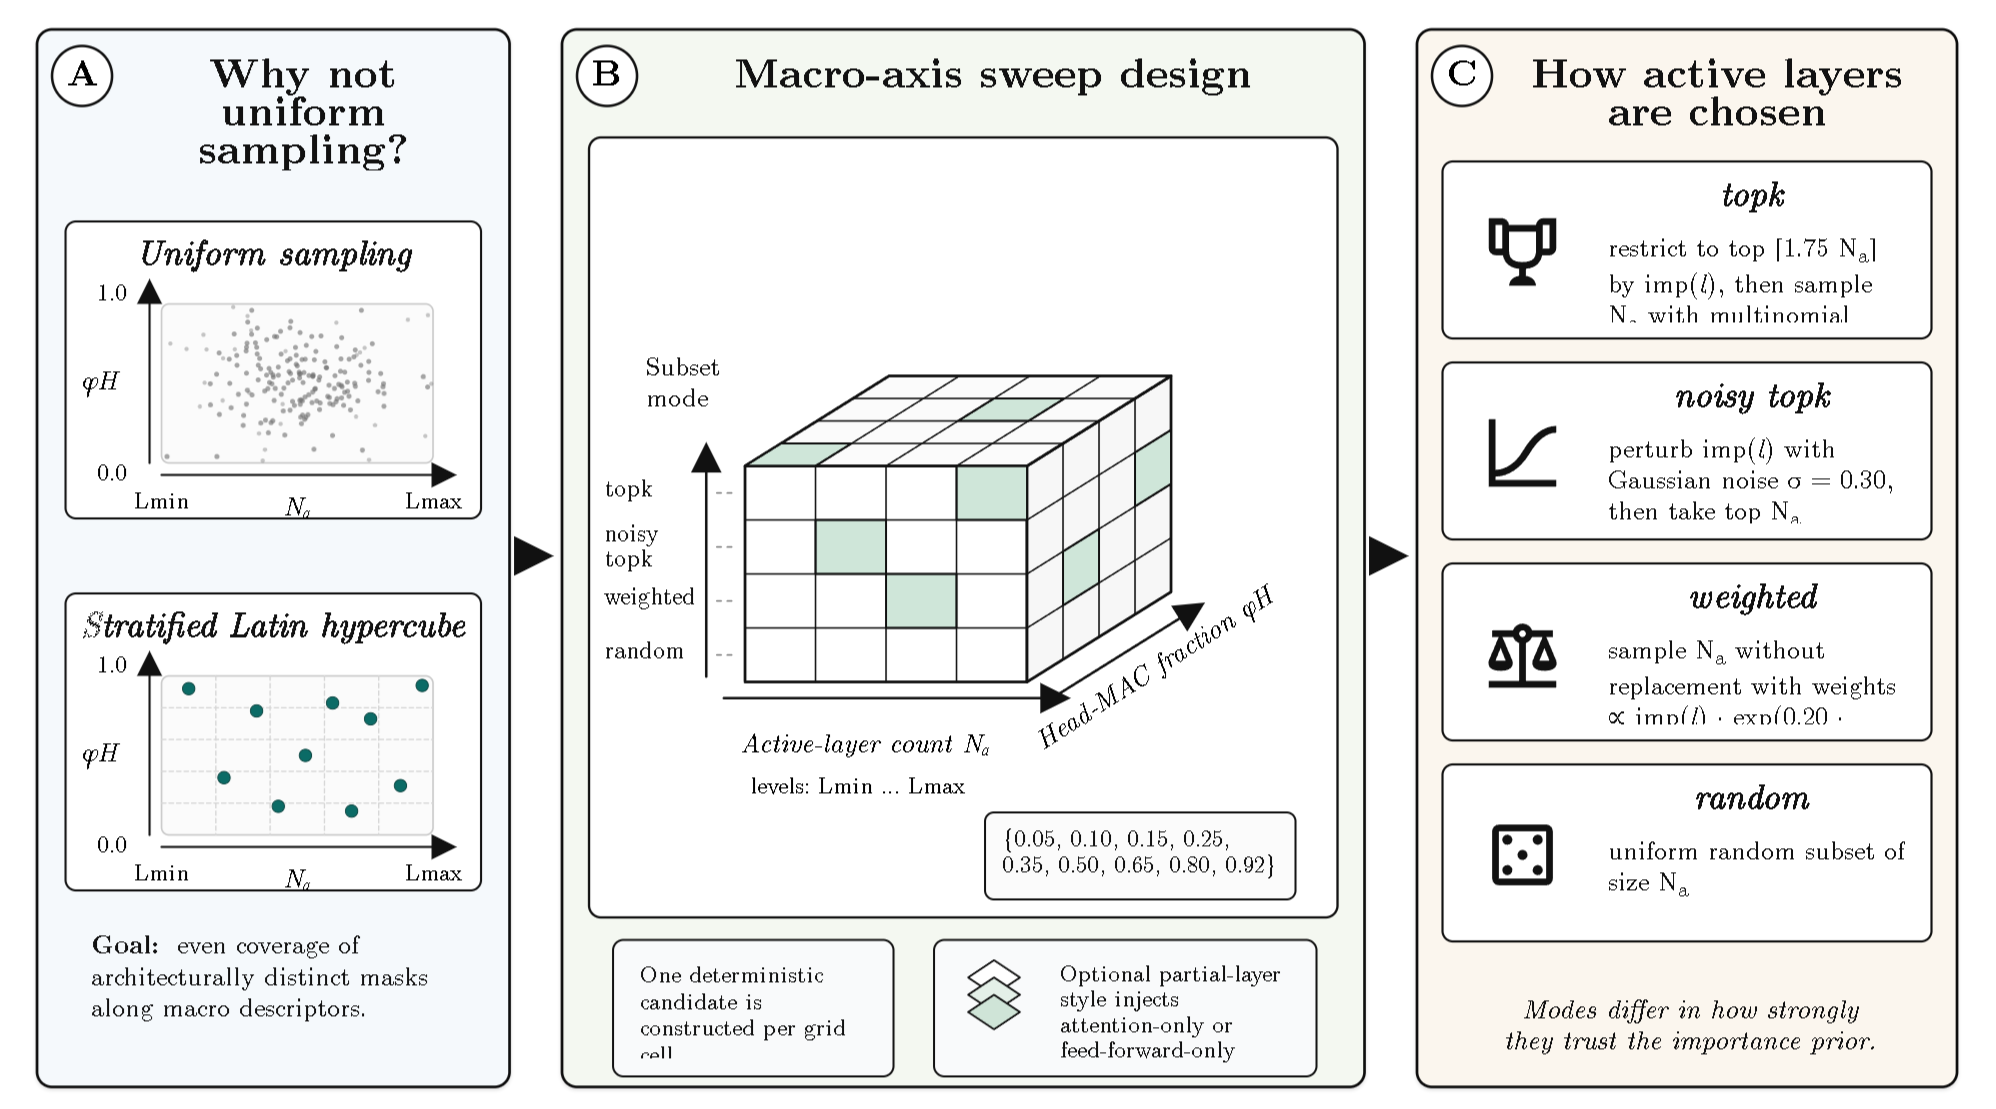
\includegraphics[width=0.95\linewidth]{figures/sweep_lhs.png}
\caption{Structure-aware sweep. Each cell of the three-axis grid $(\nactive, \phi_H, \mathrm{mode})$ yields one candidate. The subset mode chooses the active layers from $\mathrm{imp}(\ell)$; the head--neuron split $\phi_H$ divides the budget; and the importance-weighted per-layer allocation distributes the split into integer head counts and block-aligned neuron counts.}
\label{fig:sweep_lhs}
\end{figure}

A candidate produced this way is feasible by construction up to rounding and clipping, but the rounding of head counts and the floor on neuron blocks can leave its operation cost just outside the band. The candidate is therefore projected into $\mathcal{X}_\budget$ by the budget repair, which adds or removes blocks until the cost lies in the feasibility band. Repeating the construction over every cell of the grid yields a pool of approximately $300$ feasible candidates whose macro descriptors span the grid, which feeds Phase~3 in two ways: as the seed material from which the per-region populations are drawn, and as the sample on which the partition of $\mathcal{X}_\budget$ into regions is fitted.


\subsection{CVT Partition and Island Construction}
\label{detailed:cvt}

\begin{figure}[h]
\centering
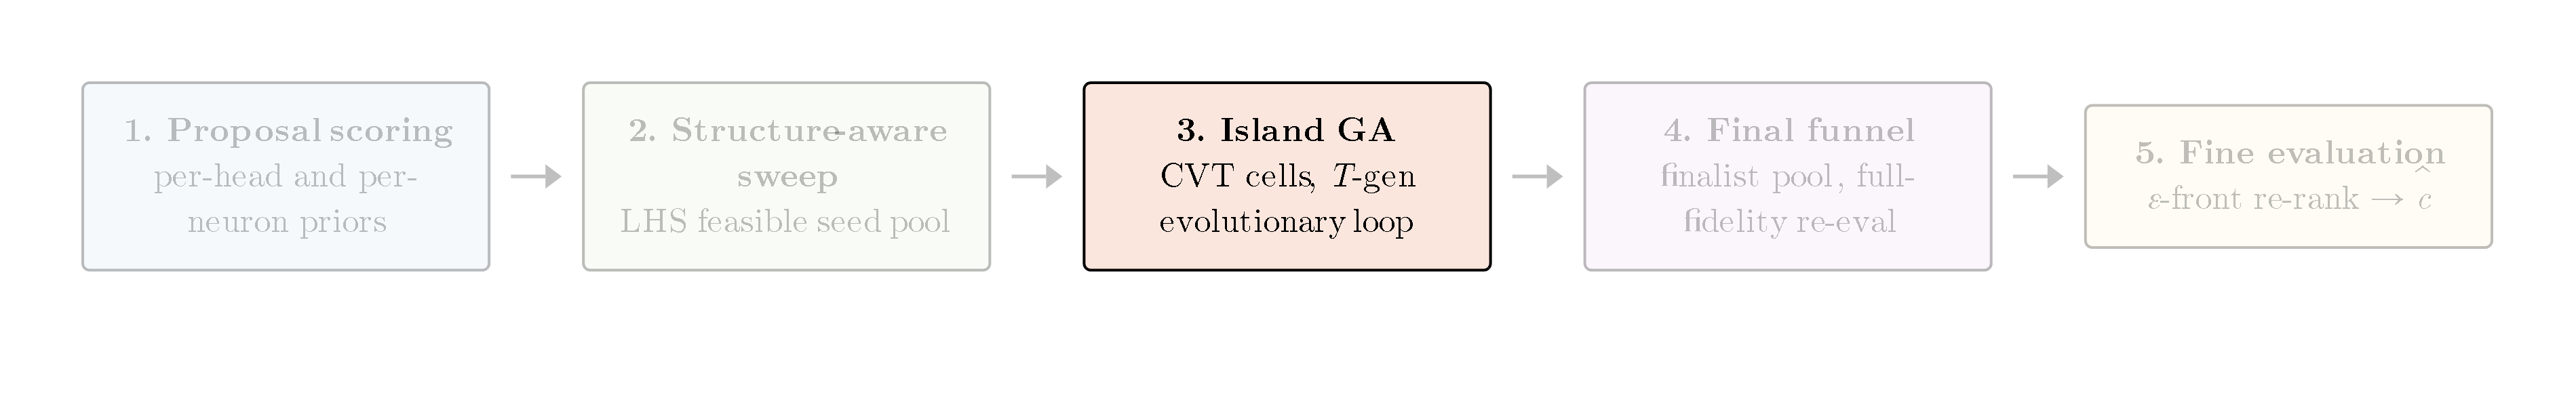
\includegraphics[width=0.85\linewidth]{figures/phase_banner_3.png}
\end{figure}

The sweep returns a pool of feasible candidates that already spans the budget band along several macro axes, but it does not yet group them into archetypes. The third phase needs such a grouping: each per-region population should sit inside one architecturally coherent neighbourhood so that its operators refine a single shape rather than averaging across incompatible ones. The grouping is obtained by clustering the sweep pool in a six-coordinate behavioural descriptor, then using each cluster as a basin in which one population evolves.

\paragraph{The architectural descriptor.}
For a candidate $\cand$ define the descriptor $z(\cand) = (z_1, \ldots, z_6) \in [0, 1]^6$ whose six coordinates capture independent macro properties of the mask. Let $\actl, \nactl$ denote the active head count and neuron count at layer $\ell$, $\headcost, \neuroncost$ the per-head and per-neuron operation costs, and $H_{\mathrm{tot}} = \sum_\ell \actl$, $N_{\mathrm{tot}} = \sum_\ell \nactl$. The first coordinate is the share of the candidate's operation cost spent on attention,
\[
z_1(\cand) \;=\; \frac{H_{\mathrm{tot}} \,\headcost}{H_{\mathrm{tot}} \,\headcost + N_{\mathrm{tot}} \,\neuroncost},
\]
and separates head-dominated masks from neuron-dominated ones. The second coordinate is the neuron fraction of the dense capacity,
\[
z_2(\cand) \;=\; \frac{N_{\mathrm{tot}}}{\nlayers \, \nffn},
\]
and measures how much of the feed-forward width survives across all layers. The third coordinate is the fraction of layers that retain at least one head and at least one neuron block,
\[
z_3(\cand) \;=\; \frac{|\{\ell : \actl > 0 \,\wedge\, \nactl > 0\}|}{\nlayers},
\]
and distinguishes deep masks (most layers active) from shallow ones (many layers dropped). The fourth coordinate measures how evenly the budget is spread across active depth by the normalised entropy
\[
z_4(\cand) \;=\; -\frac{1}{\log \nlayers} \sum_{\ell : b_\ell > 0} p_\ell \log p_\ell, \qquad p_\ell \;=\; \frac{b_\ell}{\sum_k b_k}, \quad b_\ell \;=\; \actl \,\headcost + \nactl \,\neuroncost,
\]
which is one for a perfectly uniform per-layer budget and small for a budget concentrated in a few layers. The last two coordinates locate the centre of mass of attention and of neurons along the depth axis,
\[
z_5(\cand) \;=\; \frac{1}{(\nlayers - 1) H_{\mathrm{tot}}} \sum_{\ell} \ell \cdot \actl, \qquad
z_6(\cand) \;=\; \frac{1}{(\nlayers - 1) N_{\mathrm{tot}}} \sum_{\ell} \ell \cdot \nactl,
\]
so a mask with attention concentrated in the lower layers has small $z_5$ and one with attention in the upper layers has large $z_5$. Each coordinate is clipped to $[0,1]$. The six coordinates are by construction comparable across candidates of equal cost: two masks with the same $\macop$ but different shape produce noticeably different descriptors, and two masks that differ only by a budget-neutral swap produce nearly identical descriptors.

\paragraph{Standardisation.}
The descriptors are clustered after standardisation. Writing $z_i = z(\cand_i)$ for the sweep candidates $\cand_1, \ldots, \cand_M$ and
\[
\bar z \;=\; \frac{1}{M} \sum_{i=1}^{M} z_i, \qquad \sigma_z \;=\; \mathrm{std}(z_1, \ldots, z_M),
\]
the standardised descriptors are $\tilde z_i = (z_i - \bar z) / \sigma_z$ (componentwise). Standardisation puts all six coordinates on a common scale, so the clustering does not implicitly weight, say, $z_4$ above $z_1$ just because $z_4$ has the wider raw range on this sample.

\paragraph{Initialisation by farthest-point seeding.}
The cluster centres are initialised by a deterministic variant of the $k$-means++ rule. The first centre $\tilde \mu_1$ is drawn uniformly at random from $\{\tilde z_i\}$; thereafter the next centre is the point that maximises its squared distance to the closest existing centre,
\[
\tilde \mu_{c+1} \;=\; \arg\max_{\tilde z_i} \;\min_{1 \le j \le c} \|\tilde z_i - \tilde \mu_j\|_2^{\,2}.
\]
This farthest-point construction guarantees that each new centre is placed in the part of the descriptor space least covered by the existing centres, which avoids the degenerate behaviour of uniform random initialisation when the sweep pool contains several visually similar clusters.

\paragraph{Lloyd iterations.}
Given the seeded centres, the assignment and update steps of Lloyd's algorithm alternate until the assignments stabilise. The assignment step sends each $\tilde z_i$ to the nearest centre,
\[
\mathrm{label}(i) \;=\; \arg\min_{1 \le c \le k} \|\tilde z_i - \tilde \mu_c\|_2^{\,2},
\]
and the update step replaces each centre by the mean of the points assigned to it,
\[
\tilde \mu_c \;\leftarrow\; \frac{1}{|C_c|} \sum_{i \in C_c} \tilde z_i, \qquad C_c \;=\; \{i : \mathrm{label}(i) = c\}.
\]
The iteration is run until $\mathrm{label}(\cdot)$ and the centres no longer change (in our default configuration, at most thirty Lloyd steps; the typical fixed point is reached within ten). The output is a label vector $\mathrm{label}(\cdot)$ and a set of centres $\{\tilde \mu_c\}_{c=1}^{k}$, which are mapped back to the unstandardised descriptor coordinates by $\mu_c = \sigma_z \tilde \mu_c + \bar z$.

\paragraph{Voronoi cells and the partition.}
The partition of the descriptor space follows from the centres without any further computation. Each cell $V_c$ is the set of descriptor vectors closer to $\mu_c$ than to any other centre,
\[
V_c \;=\; \big\{z \in [0,1]^6 :\, \|z - \mu_c\|_2 \le \|z - \mu_{c'}\|_2 \;\text{for all}\; c' \neq c\big\},
\]
and the cells $\{V_c\}_{c=1}^{k}$ form a centroidal Voronoi tessellation of the descriptor space. Because Lloyd's algorithm at a fixed point produces centres that are the centroids of their own cells, the partition has the property that each cell is exactly balanced against its centre under the empirical distribution of the sweep, which is what makes the partition behave well when the descriptor distribution is non-uniform.

\paragraph{BasinSpec.}
A cell is not just a region of descriptor space; it is also a region of mask space, since a candidate is feasible if and only if its mask satisfies a small number of integer constraints on heads, neurons, and layer counts. For each cell $c$ we therefore derive a BasinSpec, which translates the cell's descriptor region into a concrete range of admissible $(\actl, \nactl)$ allocations,
\[
\mathcal{B}_c \;=\; \big(\, h^c_{\min}, h^c_{\max},\; n^c_{\min}, n^c_{\max},\; [\phi^c_-, \phi^c_+],\; [u^c_-, u^c_+],\; \rho^c_{\min},\; \mu_c,\; r_c \,\big).
\]
The bounds are derived from quantiles of the sweep candidates assigned to cell $c$. Concretely, $(h^c_{\min}, h^c_{\max})$ are the empirical $5$th and $95$th percentiles of $H_{\mathrm{tot}}$ over the cell's members, $(n^c_{\min}, n^c_{\max})$ are the corresponding block-aligned percentiles of $N_{\mathrm{tot}}$, $[\phi^c_-, \phi^c_+]$ is the $10$th--$90$th percentile band of $z_1$ in the cell, $[u^c_-, u^c_+]$ is a similar band on per-layer utilisation, $\rho^c_{\min}$ is a floor on the operation cost as a fraction of the budget, and $r_c$ is the $75$th percentile of $\|\tilde z_i - \tilde \mu_c\|_2$ over $i \in C_c$ (the cell's effective radius in standardised space). The BasinSpec is the object that the basin projection of the search uses to enforce feasibility against the cell's structural region during Phase~3.

\paragraph{One population per basin.}
Each basin hosts one population $\pop_c$ of fixed size $P$. The population is seeded from the sweep pool: every sweep candidate already assigned to cell $c$ is included as a candidate seed, and any remaining slots are filled by drawing candidates from neighbouring cells and projecting them into $\mathcal{B}_c$. The projection adjusts the head and neuron counts to lie within $(h^c_{\min}, h^c_{\max})$, $(n^c_{\min}, n^c_{\max})$, and $[\phi^c_-, \phi^c_+]$, and then runs the budget repair to bring the operation cost back into the feasibility band. The result is a population whose members all satisfy the basin's constraints and whose collective coverage of the cell is balanced; subsequent generations refine the population in place without leaving the cell.

\paragraph{Archetypes in the sweep pool.}
Empirically the descriptors of the sweep candidates concentrate in a small number of recognisable shapes, and the partition consistently produces five archetypal basins. The \emph{head-heavy with few neurons} archetype carries a large $z_1$ (head MAC share above $\sim 0.7$) and a small $z_2$, modelling masks that bet their budget on attention and prune the feed-forward stacks. The \emph{head-leaning with mid neurons} archetype keeps a head MAC share in the $0.5$--$0.78$ band and the neuron fraction in a middle range, modelling balanced architectures with a head bias. The \emph{balanced} archetype sits in the middle of both $z_1$ and $z_2$ and matches the dense-like masks. The \emph{neuron-heavy} archetype mirrors the first: low $z_1$ (below $\sim 0.32$) and high $z_2$, modelling feed-forward-dominated masks. The \emph{layer-sparse} archetype is defined less by the head-versus-neuron split and more by $z_3$: it consists of masks that keep only a few layers active but allocate a large head MAC share to them, modelling deep-narrow versus shallow-wide architectures within the same budget. The five archetypes provide qualitatively different starting points for Phase~3, and the search relies on them to explore qualitatively different shapes in parallel.

\begin{figure}[h]
\centering
\includegraphics[width=0.95\linewidth]{figures/cvt_partition.png}
\caption{CVT partition of the descriptor space, shown in the $(z_1, z_3)$ plane (head MAC share versus active-layer fraction). Sweep candidates appear as dots, the five Voronoi cells are drawn as shaded polygons with their centroids $\mu_c$, and each cell is labelled with the archetype it concentrates. One population is seeded in each cell from the sweep candidates assigned to it.}
\label{fig:cvt_partition}
\end{figure}
